\documentclass{article}
% generated by Madoko, version 1.0.0-rc5
%mdk-data-line={1}


\usepackage[heading-base={2},section-num={False},bib-label={True}]{madoko2}


\begin{document}



%mdk-data-line={8}
\mdxtitleblockstart{}
%mdk-data-line={8}
\mdxtitle{\mdline{8}Optimization of a DNN Program on the CPU+MIC Platform}%mdk

%mdk-data-line={11}
\mdxsubtitle{\mdline{11}Competition proposal of ASC}%mdk

%mdk-data-line={14}
\mdxtitlenote{\mdline{14}2016-02-26}%mdk
\mdxauthorstart{}
%mdk-data-line={19}
\mdxauthorname{\mdline{19}University of Electronic Secience and Technology of China}%mdk
\mdxauthorend\mdtitleauthorrunning{}{}\mdxtitleblockend%mdk

%mdk-data-line={10}
\begin{abstract}%mdk

%mdk-data-line={11}
\noindent\mdline{11}This article is a part of competition proposal of Asia Supercomputer Student Challenge. We analysis the \mdline{11}\mdcode{DNN}\mdline{11} program, discuss different design methods, and show optimization methods with their efforts.%mdk
%mdk
\end{abstract}%mdk
\mdline{14}
\begin{mdtoc}%mdk

\section*{Contents}\label{sec-contents}%mdk%mdk

\begin{mdtocblock}%mdk

\mdtocitemx{sec-introduction}{\mdref{sec-introduction}{1.\hspace*{0.5em}Introduction}}%mdk

\mdtocitemx{sec-analysis-of-the-serial-program}{\mdref{sec-analysis-of-the-serial-program}{2.\hspace*{0.5em}Analysis of the Serial Program}}%mdk

\begin{mdtocblock}%mdk

\mdtocitemx{sec-coarse-grain-analysis}{\mdref{sec-coarse-grain-analysis}{2.1.\hspace*{0.5em}Coarse Grain Analysis}}%mdk

\mdtocitemx{sec-fine-grain-analysis}{\mdref{sec-fine-grain-analysis}{2.2.\hspace*{0.5em}Fine Grain Analysis}}%mdk

\begin{mdtocblock}%mdk

\mdtocitemx{sec-matrix-size}{\mdref{sec-matrix-size}{2.2.1.\hspace*{0.5em}Matrix Size}}%mdk

\mdtocitemx{sec-cycles-index}{\mdref{sec-cycles-index}{2.2.2.\hspace*{0.5em}Cycles Index}}%mdk
%mdk
\end{mdtocblock}%mdk
%mdk
\end{mdtocblock}%mdk

\mdtocitemx{sec-parallelization-design-methods}{\mdref{sec-parallelization-design-methods}{3.\hspace*{0.5em}Parallelization Design Methods}}%mdk

\begin{mdtocblock}%mdk

\mdtocitemx{sec-fine-grain-parallelism}{\mdref{sec-fine-grain-parallelism}{3.1.\hspace*{0.5em}Fine Grain Parallelism}}%mdk

\mdtocitemx{sec-coarse-grain-parallelism}{\mdref{sec-coarse-grain-parallelism}{3.2.\hspace*{0.5em}Coarse Grain Parallelism}}%mdk
%mdk
\end{mdtocblock}%mdk

\mdtocitemx{sec-performance-optimization-methods}{\mdref{sec-performance-optimization-methods}{4.\hspace*{0.5em}Performance Optimization Methods}}%mdk

\begin{mdtocblock}%mdk

\mdtocitemx{sec-compiler-assisted-offload}{\mdref{sec-compiler-assisted-offload}{4.1.\hspace*{0.5em}Compiler Assisted Offload}}%mdk

\begin{mdtocblock}%mdk

\mdtocitemx{sec-scope-of-offloaded-sections}{\mdref{sec-scope-of-offloaded-sections}{4.1.1.\hspace*{0.5em}Scope of Offloaded Sections}}%mdk

\mdtocitemx{sec-dimensionality-reduction}{\mdref{sec-dimensionality-reduction}{4.1.2.\hspace*{0.5em}Dimensionality Reduction}}%mdk
%mdk
\end{mdtocblock}%mdk

\mdtocitemx{sec-openmp-optimization}{\mdref{sec-openmp-optimization}{4.2.\hspace*{0.5em}\mdcode{OpenMP} Optimization}}%mdk

\mdtocitemx{sec-alignment}{\mdref{sec-alignment}{4.3.\hspace*{0.5em}Alignment}}%mdk

\mdtocitemx{sec-environmental-variables-settings}{\mdref{sec-environmental-variables-settings}{4.4.\hspace*{0.5em}Environmental Variables Settings}}%mdk

\begin{mdtocblock}%mdk

\mdtocitemx{sec-mkl_dynamictrue-}{\mdref{sec-mkl_dynamictrue-}{4.4.1.\hspace*{0.5em}\mdcode{MKL\_DYNAMIC=true}:}}%mdk

\mdtocitemx{sec-mkl_num_threads57-omp_num_threads57-}{\mdref{sec-mkl_num_threads57-omp_num_threads57-}{4.4.2.\hspace*{0.5em}\mdcode{MKL\_NUM\_THREADS=57~OMP\_NUM\_THREADS=57}:}}%mdk

\mdtocitemx{sec-mic_use_2mb_buffers64k}{\mdref{sec-mic_use_2mb_buffers64k}{4.4.3.\hspace*{0.5em}\mdcode{MIC\_USE\_2MB\_BUFFERS=64K}}}%mdk
%mdk
\end{mdtocblock}%mdk
%mdk
\end{mdtocblock}%mdk

\mdtocitemx{sec-testing-process-and-results-on-the-cpumic-platform}{\mdref{sec-testing-process-and-results-on-the-cpumic-platform}{5.\hspace*{0.5em}Testing Process and Results on the CPU+MIC Platform}}%mdk

\mdtocitemx{sec-bibliography}{\mdref{sec-bibliography}{References}}%mdk
%mdk
\end{mdtocblock}%mdk
%mdk
\end{mdtoc}%mdk

%mdk-data-line={16}
\section{\mdline{16}1.\hspace*{0.5em}\mdline{16}Introduction}\label{sec-introduction}%mdk%mdk

%mdk-data-line={17}
\noindent\mdline{17}There is a program based on a standalone hybrid CPU+MIC platform called \mdline{17}\mdcode{DNN(deep~neural~network)}\mdline{17} needed to be parallelized for obtain better performance. We could use any parallel programming mode supported by \mdline{17}\mdcode{MIC}\mdline{17} to achieve this goal. Here is some detailed information about hardware in Figure 1, software configuration in Figure 2.%mdk

%mdk-data-line={19}
\mdline{19}After optimization, the final program is tested on one computing server on the CPU+MIC hybrid cluster. Performance analysis in this proposal is based on the results of this test.%mdk

%mdk-data-line={20}
\begin{figure}[tbp]%mdk
\begin{mdcenter}%mdk

%mdk-data-line={22}
\noindent\mdline{22}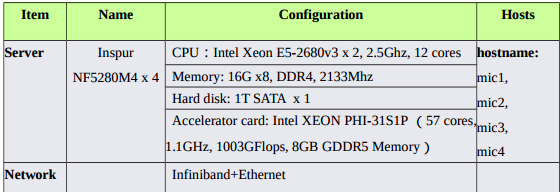
\includegraphics[keepaspectratio=true,width=\dimmin{}{\dimwidth{0.90}}]{images/2016-02-18-23-01-13-}{}\mdline{22}%mdk

%mdk-data-line={25}
\mdhr{}%mdk

%mdk-data-line={26}
\noindent\mdline{26}\mdcaption{\textbf{Figure~\mdcaptionlabel{1}.}~\mdcaptiontext{Hardware configuration}}%mdk
%mdk
\end{mdcenter}\label{fig-myfigure}%mdk
%mdk
\end{figure}%mdk

%mdk-data-line={27}
\begin{figure}[tbp]%mdk
\begin{mdcenter}%mdk

%mdk-data-line={28}
\noindent\mdline{28}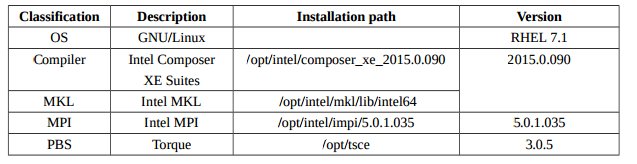
\includegraphics[keepaspectratio=true,width=\dimmin{}{\dimwidth{0.90}}]{images/2016-02-18-23-13-11-}{}\mdline{28}%mdk

%mdk-data-line={31}
\mdhr{}%mdk

%mdk-data-line={32}
\noindent\mdline{32}\mdcaption{\textbf{Figure~\mdcaptionlabel{2}.}~\mdcaptiontext{Software configuration}}%mdk
%mdk
\end{mdcenter}\label{fig-myfigure}%mdk
%mdk
\end{figure}%mdk

%mdk-data-line={33}
\section{\mdline{33}2.\hspace*{0.5em}\mdline{33}Analysis of the Serial Program}\label{sec-analysis-of-the-serial-program}%mdk%mdk

%mdk-data-line={34}
\subsection{\mdline{34}2.1.\hspace*{0.5em}\mdline{34}Coarse Grain Analysis}\label{sec-coarse-grain-analysis}%mdk%mdk

%mdk-data-line={35}
\noindent\mdline{35}At first, we generate a call graph(Figure 3) by using \mdline{35}\mdcode{Google~perfools}\mdline{35}, a open source performance profiler, to have a glance though it. Every square represents a function, and the bigger square is, the more time corresponding function costs.%mdk

%mdk-data-line={37}
\begin{figure}[tbp]%mdk
\begin{mdcenter}%mdk

%mdk-data-line={38}
\noindent\mdline{38}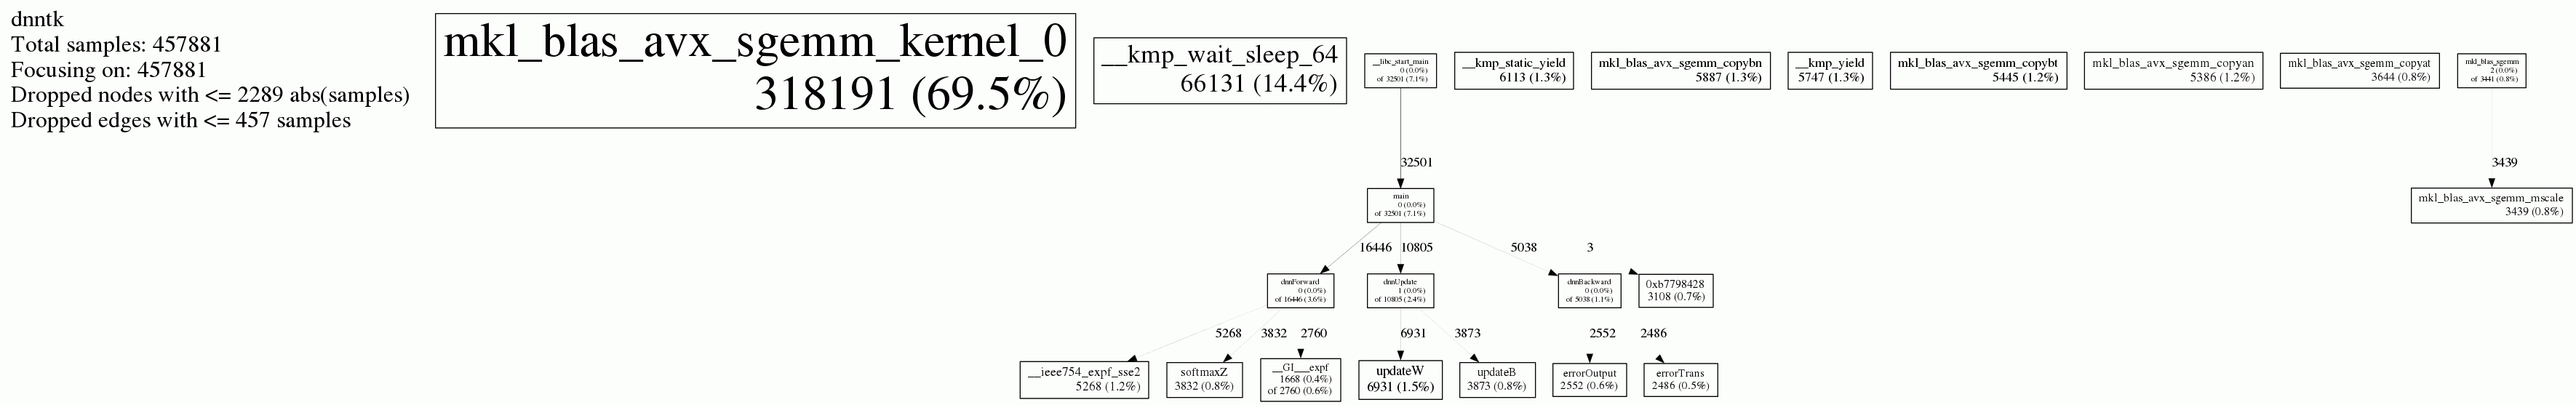
\includegraphics[keepaspectratio=true,width=\dimmin{}{\dimwidth{0.90}}]{images/100001994364201}{}\mdline{38}%mdk

%mdk-data-line={41}
\mdhr{}%mdk

%mdk-data-line={42}
\noindent\mdline{42}\mdcaption{\textbf{Figure~\mdcaptionlabel{3}.}~\mdcaptiontext{Google Perfools results}}%mdk
%mdk
\end{mdcenter}\label{fig-myfigure}%mdk
%mdk
\end{figure}%mdk

%mdk-data-line={42}
\mdline{42}Obviously, the hot spot is something about \mdline{42}\mdcode{MKL}\mdline{42}. After googling
and searching Intel document we know that MKL provides \mdline{43}\mdcode{BLAS~routinues}\mdline{43}, which includes a serial function named \mdline{43}\mdcode{cblas\_?gemm}\mdline{43} to compute a product of general matrices.%mdk

%mdk-data-line={45}
\mdline{45}But giving that MKL function is well-optimized\mdline{45}[\mdcite{sgemm}{4}]\mdline{45}, we search for all position where \mdline{45}\mdcode{cblas\_*gemm}\mdline{45} is called. Results show the usage of \mdline{45}\mdcode{cblas\_*gemm}\mdline{45} appear in file \mdline{45}\mdcode{dnn\_func.cpp}\mdline{45}, more specifically, in three functions:%mdk

%mdk-data-line={47}
\begin{itemize}[noitemsep,topsep=\mdcompacttopsep]%mdk

%mdk-data-line={47}
\item\mdline{47}\mdcode{\preindent{1}extern~"C"~int~dnnForward(NodeArg~\&nodeArg)}\mdline{47}%mdk

%mdk-data-line={48}
\item\mdline{48}\mdcode{\preindent{1}extern~"C"~int~dnnBackward(NodeArg~\&nodeArg)}\mdline{48}%mdk

%mdk-data-line={49}
\item\mdline{49}\mdcode{\preindent{1}extern~"C"~int~dnnUpdate(NodeArg~\&nodeArg)}\mdline{49}%mdk
%mdk
\end{itemize}%mdk

%mdk-data-line={51}
\begin{figure}[tbp]%mdk
\begin{mdcenter}%mdk

%mdk-data-line={52}
\noindent\mdline{52}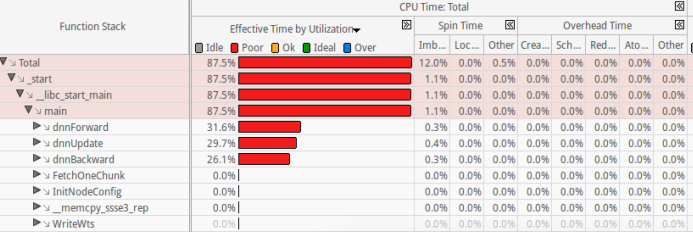
\includegraphics[keepaspectratio=true,width=\dimmin{}{\dimwidth{0.90}}]{images/2016-02-19-10-36-25-}{}\mdline{52}%mdk

%mdk-data-line={54}
\mdhr{}%mdk

%mdk-data-line={55}
\noindent\mdline{55}\mdcaption{\textbf{Figure~\mdcaptionlabel{4}.}~\mdcaptiontext{Intel VTune top-down tree}}%mdk
%mdk
\end{mdcenter}\label{fig-myfigure}%mdk
%mdk
\end{figure}%mdk

%mdk-data-line={56}
\noindent\mdline{56}They call \mdline{56}\mdcode{MKL}\mdline{56} function \mdline{56}\mdcode{cblas\_sgemm}\mdline{56} many times in their \mdline{56}\mdcode{for~loop}\mdline{56} and 
cost almost 90\% of all CPU time. So we guess that those function
 is what we may optimize, aka, hotspots. The report(see Figure 4.) showed by\mdline{58}\mdcode{Intel~VTune}\mdline{58}, another profiler, proves our guess.%mdk

%mdk-data-line={60}
\mdline{60}According to a skim through the source code, we could establish a clear structure about this program. To simplify code, original program could be rewritten in pseudocode:%mdk
\begin{mdpre}%mdk
\noindent~~~{\mdcolor{teal}GetInitFileConfig}(cpuArg)\\
~~~{\mdcolor{teal}While}~{\mdcolor{teal}FetchOneChunk}(cpuArg,~onChunk)~{\mdcolor{navy}do}:\\
~~~~~~~~~~~{\mdcolor{teal}While}~{\mdcolor{teal}FetchOneBunch}(oneChunk,~nodeArg)~{\mdcolor{navy}do}:\\
~~~~~~~~~~~~~~~~dnnForward(nodeArg)\\
~~~~~~~~~~~~~~~~dnnBackward(nodeArg)\\
~~~~~~~~~~~~~~~~dnnUpate(nodeArg)\\
~~~~{\mdcolor{teal}WriteWts}(nodeArg,~cpuArg)\\
~~~~{\mdcolor{teal}UninitProgramConfig}(cpuArg)\\
%mdk
\end{mdpre}\noindent\mdline{72}There are two nested loop surrounding \mdline{72}\mdcode{dnn*()}\mdline{72} series, and 
in each of those processing function some matrix-matrix product are
calculated. Whether those hotspots could be parallelized or not depends
on data scale, dependency and so on. Before we discuss some methods and weighed their pros and cons the implementation of \mdline{75}\mdcode{DNN}\mdline{75} should be carefully checked.

%mdk-data-line={77}
\subsection{\mdline{77}2.2.\hspace*{0.5em}\mdline{77}Fine Grain Analysis}\label{sec-fine-grain-analysis}%mdk%mdk

%mdk-data-line={79}
\subsubsection{\mdline{79}2.2.1.\hspace*{0.5em}\mdline{79}Matrix Size}\label{sec-matrix-size}%mdk%mdk

%mdk-data-line={80}
\noindent\mdline{80}Here is an example of how \mdline{80}\mdcode{DNN}\mdline{80} use \mdline{80}\mdcode{cblas\_sgemm}\mdline{80}:%mdk
\begin{mdpre}%mdk
\noindent~~cblas\_sgemm({\mdcolor{teal}CblasRowMajor},~{\mdcolor{teal}CblasNoTrans},~{\mdcolor{teal}CblasNoTrans},\textbackslash{}\\
~~~~~~~~numN,~numA[i],~numA[i-{\mdcolor{purple}1}],~\textbackslash{}\\
~~~~~~~~one,~d\_Y[i-{\mdcolor{purple}1}],~numA[i-{\mdcolor{purple}1}],~d\_W[i],~numA[i],\\
~~~~~~~~one,~d\_Y[i],~numA[i]);%mdk
\end{mdpre}\noindent\mdline{88}In this way we could calculate \mdline{88}\mdcode{d\_Y[i-1]}\mdline{88} \mdline{88}*\mdline{88} \mdline{88}\mdcode{d\_W[i]}\mdline{88} \mdline{88}+ \mdline{88}\mdcode{d\_Y[i]}\mdline{88} and assign the result to \mdline{88}\mdcode{d\_Y[i]}\mdline{88}. The arguments \mdline{88}\mdcode{numN}\mdline{88}, \mdline{88}\mdcode{numA[i]}\mdline{88}, \mdline{88}\mdcode{numA[i-1]}\mdline{88} indicating the size of the matrices:

%mdk-data-line={90}
\begin{itemize}[noitemsep,topsep=\mdcompacttopsep]%mdk

%mdk-data-line={90}
\item\mdline{90}\mdcode{d\_Y[i-1]}\mdline{90} is a \mdline{90}\mdcode{numN}\mdline{90} row by \mdline{90}\mdcode{numA[i]}\mdline{90} column matrix;%mdk

%mdk-data-line={91}
\item\mdline{91}\mdcode{d\_W[i]}\mdline{91} is a \mdline{91}\mdcode{numN}\mdline{91} row by \mdline{91}\mdcode{numA[i-1]}\mdline{91} column matrix;%mdk

%mdk-data-line={92}
\item\mdline{92}\mdcode{d\_Y[i]}\mdline{92} is a \mdline{92}\mdcode{numA[i-1]}\mdline{92} row by \mdline{92}\mdcode{numA[i]}\mdline{92} column matrix.%mdk
%mdk
\end{itemize}%mdk

%mdk-data-line={94}
\noindent\mdline{94}As we known the bigger matrix size is, the higher degree of \mdline{94}\mdcode{MKL}\mdline{94} parallelism is\mdline{94}[\mdcite{paramkl}{5}]\mdline{94}. But in the \mdline{94}\mdcode{DNN}\mdline{94} program, the size of matrix is decided by \mdline{94}\mdcode{bunchSize}\mdline{94}, a constant integer (\mdline{94}\ensuremath{\approx}\mdline{94}1024), and a element (\mdline{94}\ensuremath{\approx}\mdline{94}1024) of \mdline{94}\mdcode{dnnLayerArr}\mdline{94}, which is a constant integer array. The two integers are set by configuration file, and we are not allowed to modify it. For this reason there are no sufficiently large matrix to enable \mdline{94}\mdcode{auto~offload~model}\mdline{94} of \mdline{94}\mdcode{MIC}\mdline{94} to speed up \mdline{94}\mdcode{DNN}\mdline{94}.\mdline{94}[\mdcite{mkl-mic}{2}]\mdline{94}%mdk

%mdk-data-line={96}
\subsubsection{\mdline{96}2.2.2.\hspace*{0.5em}\mdline{96}Cycles Index}\label{sec-cycles-index}%mdk%mdk

%mdk-data-line={97}
\noindent\mdline{97}In the \mdline{97}\mdcode{dnn*}\mdline{97} series every loop call \mdline{97}\mdcode{cblas\_sgemm}\mdline{97} \mdline{97}\mdcode{numN}\mdline{97}(\mdline{97}\ensuremath{\approx}\mdline{97}7) times, which indicates the length of \mdline{97}\mdcode{dnnLayerArr}\mdline{97}. It\mdline{97}'\mdline{97}s regretful that the value also cannot be modified by us. Giving the number of core(\mdline{97}\ensuremath{\approx}\mdline{97}24 on CPU or \mdline{97}\ensuremath{\approx}\mdline{97}60 on MIC) and constant \mdline{97}\mdcode{numN}\mdline{97}, we couldn\mdline{97}'\mdline{97}t improve performance a lot by parallelizing those loops.%mdk

%mdk-data-line={99}
\section{\mdline{99}3.\hspace*{0.5em}\mdline{99}Parallelization Design Methods}\label{sec-parallelization-design-methods}%mdk%mdk

%mdk-data-line={101}
\subsection{\mdline{101}3.1.\hspace*{0.5em}\mdline{101}Fine Grain Parallelism}\label{sec-fine-grain-parallelism}%mdk%mdk

%mdk-data-line={102}
\begin{figure}[tbp]%mdk
\begin{mdcenter}%mdk

%mdk-data-line={103}
\noindent\mdline{103}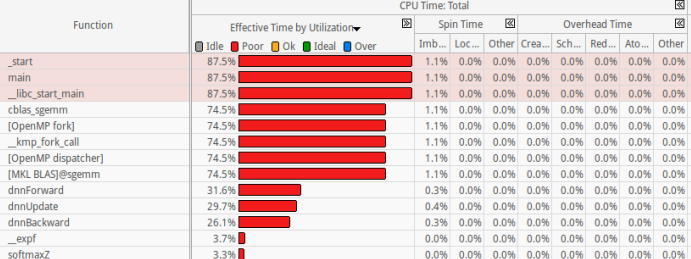
\includegraphics[keepaspectratio=true,width=\dimmin{}{\dimwidth{0.90}}]{images/2016-02-19-10-36-48-}{}\mdline{103}%mdk

%mdk-data-line={105}
\mdhr{}%mdk

%mdk-data-line={106}
\noindent\mdline{106}\mdcaption{\textbf{Figure~\mdcaptionlabel{5}.}~\mdcaptiontext{Overview of consumed time}}%mdk
%mdk
\end{mdcenter}\label{fig-figure}%mdk
%mdk
\end{figure}%mdk

%mdk-data-line={106}
\noindent\mdline{106}From the figure above it\mdline{106}'\mdline{106}s easy to find that \mdline{106}\mdcode{dnn*}\mdline{106} series, which invoke \mdline{106}\mdcode{cblas\_sgemm}\mdline{106} many times in \mdline{106}\mdcode{for~loop}\mdline{106}, nearly cost all CPU time. A rough thoughts occurred to us that we could parallelize those \mdline{106}\mdcode{for~loop}\mdline{106} using multi-threads. But data dependency in \mdline{106}\mdcode{for~loop}\mdline{106} and relatively small cycle index make it inefficient. So we decide to reduce the size of parallelization region. Taking the feature of \mdline{106}\mdcode{MIC}\mdline{106} in to account we hope to execute highly parallel and compute intensive code on the \mdline{106}\mdcode{MIC}\mdline{106}.\mdline{106}[\mdcite{effective_use}{3}]\mdline{106} Focusing on \mdline{106}\mdcode{dnn*}\mdline{106} series we could find an abstract structure to generalize them:%mdk
\begin{mdpre}%mdk
\noindent~~extern~{\mdcolor{maroon}"}{\mdcolor{maroon}C}{\mdcolor{maroon}"}~{\mdcolor{navy}int}~dnn***({\mdcolor{teal}NodeArg}~\&nodeArg)\\
~~\{\\
~~~~~{\mdcolor{darkgreen}/*}{\mdcolor{darkgreen}~Variables~definition~}{\mdcolor{darkgreen}*/}\\
~~~~~{\mdcolor{navy}float}~~*d\_X~=~nodeArg.d\_X;\\
~~~~~~~...\\
~~~~~~{\mdcolor{darkgreen}/*}{\mdcolor{darkgreen}~Preprcess~function~func1~}{\mdcolor{darkgreen}*/}\\
~~~~~~func1(...);\\
\\
~~~~{\mdcolor{darkgreen}/*}{\mdcolor{darkgreen}~a~for~loop~where~a~function,~a~MKL~\textbackslash{}}\\
{\mdcolor{darkgreen}~~~~and~another~function~are~invoked~oderly~}{\mdcolor{darkgreen}*/}\\
~~~~{\mdcolor{navy}for}~({\mdcolor{navy}int}~i~=~num;~...)~\{\\
~~~~~~~~~~func2(...);\\
~~~~~~~~~~cblas\_sgemm({\mdcolor{teal}CblasRowMajor},~{\mdcolor{teal}CblasNoTrans},~...);\\
~~~~~~~~~~func3(...);\\
~~~~~~~~~~\}\\
~~~~~~\}~\\
~~~~~~{\mdcolor{navy}return}~{\mdcolor{purple}0};\\
~~\}\\
%mdk
\end{mdpre}\noindent\mdline{128}Data processed by \mdline{128}\mdcode{func1}\mdline{128}, \mdline{128}\mdcode{func2}\mdline{128}, \mdline{128}\mdcode{func3}\mdline{128} are matrices or vectors, which are easy to parallelized. Taking what we discuss above into consideration, we have two choose: a) use serial \mdline{128}\mdcode{MKL}\mdline{128} then parallelize the whole \mdline{128}\mdcode{for~loop}\mdline{128}, b) use multi-thread \mdline{128}\mdcode{MKL}\mdline{128} and parallelize \mdline{128}\mdcode{func1}\mdline{128}, \mdline{128}\mdcode{func~2}\mdline{128} and \mdline{128}\mdcode{func~3}\mdline{128}. The two measures all support \mdline{128}\mdcode{MIC}\mdline{128}, but we prefer the b) because we could benefit from the parallel optimization of \mdline{128}\mdcode{MKL}\mdline{128} and cooperation among \mdline{128}\mdcode{MKL}\mdline{128} and \mdline{128}\mdcode{MIC}\mdline{128}.\mdline{128}[\mdcite{mkl-mic}{2}, \mdcite{page_file}{6}]\mdline{128}

%mdk-data-line={130}
\begin{figure}[tbp]%mdk
\begin{mdcenter}%mdk

%mdk-data-line={131}
\noindent\mdline{131}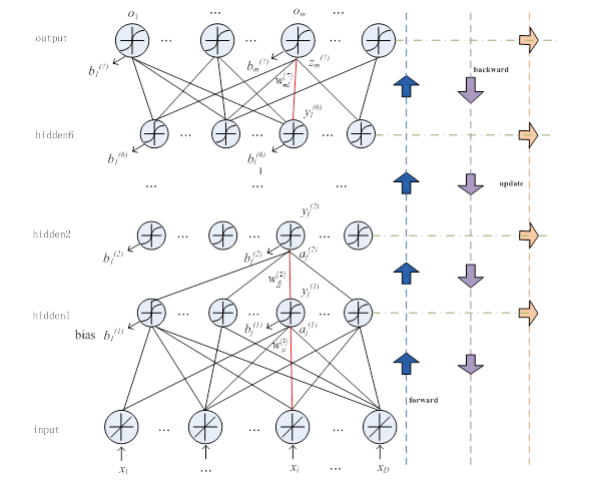
\includegraphics[keepaspectratio=true,width=\dimmin{}{\dimwidth{0.90}}]{images/2016-02-21-21-15-24-}{}\mdline{131}%mdk

%mdk-data-line={134}
\mdhr{}%mdk

%mdk-data-line={135}
\noindent\mdline{135}\mdcaption{\textbf{Figure~\mdcaptionlabel{6}.}~\mdcaptiontext{\mdcode{DNN} structure}}%mdk
%mdk
\end{mdcenter}\label{fig-figure}%mdk
%mdk
\end{figure}%mdk

%mdk-data-line={136}
\subsection{\mdline{136}3.2.\hspace*{0.5em}\mdline{136}Coarse Grain Parallelism}\label{sec-coarse-grain-parallelism}%mdk%mdk

%mdk-data-line={137}
\noindent\mdline{137}To implenment coarse grain parallelism we hope that each thread/process finish large subcomponents. To achieve this goal \mdline{137}\mdcode{DNN}\mdline{137} program should be divided into (mostly) independent and similar proportions, and every proportion should be as large as possible. But default ordering of \mdline{137}\mdcode{dnn*}\mdline{137} series couldn\mdline{137}'\mdline{137}t be changed, neither does the processing of file-reading. So in our opinion it\mdline{137}'\mdline{137}s difficult to implement coarse grain parallelism without any change to \mdline{137}\mdcode{DNN}\mdline{137} structure and its dataset. So we don\mdline{137}'\mdline{137}t plan to implement it.%mdk

%mdk-data-line={139}
\section{\mdline{139}4.\hspace*{0.5em}\mdline{139}Performance Optimization Methods}\label{sec-performance-optimization-methods}%mdk%mdk

%mdk-data-line={141}
\subsection{\mdline{141}4.1.\hspace*{0.5em}\mdline{141}Compiler Assisted Offload}\label{sec-compiler-assisted-offload}%mdk%mdk

%mdk-data-line={143}
\subsubsection{\mdline{143}4.1.1.\hspace*{0.5em}\mdline{143}Scope of Offloaded Sections}\label{sec-scope-of-offloaded-sections}%mdk%mdk

%mdk-data-line={144}
\noindent\mdline{144}We have talked about the common structure of \mdline{144}\mdcode{DNN}\mdline{144} series. In their \mdline{144}\mdcode{for}\mdline{144} loop there are processing function and \mdline{144}\mdcode{MKL}\mdline{144} function appear alternately, and the former modifies data which is used as input in \mdline{144}\mdcode{cblas\_sgemm}\mdline{144}function. Data change between \mdline{144}\mdcode{MIC}\mdline{144} and \mdline{144}\mdcode{CPU}\mdline{144} is slow because of the limitation of \mdline{144}\mdcode{PCI-E}\mdline{144} so the best known methods\mdline{144}[\mdcite{effective_use}{3}]\mdline{144} is to make the whole section of code an offload unit, which could reduce most of data transfer. In addition, if all three \mdline{144}\mdcode{dnn*}\mdline{144} function are offload units, data transfer between them is less. Then all we only need to transfer input data to \mdline{144}\mdcode{MIC}\mdline{144} before loop and fetch results. This is pseudocode of \mdline{144}\mdcode{dnn*}\mdline{144} function (issues about array transfer discussed in \mdline{144}\textquoteleft{}Dimensionality Reduction\textquoteright{}\mdline{144}):%mdk
\begin{mdpre}%mdk
\noindent~~extern~{\mdcolor{maroon}"}{\mdcolor{maroon}C}{\mdcolor{maroon}"}~{\mdcolor{navy}int}~dnn***({\mdcolor{teal}NodeArg}~\&nodeArg)\\
~~\{\\
~~~~{\mdcolor{darkgreen}/*}{\mdcolor{darkgreen}~Variables~definition~}{\mdcolor{darkgreen}*/}\\
~~~~{\mdcolor{navy}float}~~*d\_X~=~nodeArg.d\_X;\\
~~~~~~...\\
~~~~\\
~~~~\#pragma~offload~target(mic)\textbackslash{}\\
~~~~in(pd\_Y:length({\mdcolor{purple}0})~{\mdcolor{teal}REUSE})\textbackslash{}\\
~~~~in(pd\_W:length({\mdcolor{purple}0})~{\mdcolor{teal}REUSE})\textbackslash{}\\
~~~~...\\
~~~~\{\\
~~~~~~{\mdcolor{darkgreen}/*}{\mdcolor{darkgreen}~Preprcess~function~func1~}{\mdcolor{darkgreen}*/}\\
~~~~~~func1(...);\\
\\
~~~~~~{\mdcolor{darkgreen}/*}{\mdcolor{darkgreen}~a~for~loop~where~a~function,~a~MKL~\textbackslash{}}\\
{\mdcolor{darkgreen}~~~~~~and~another~function~are~invoked~oderly~}{\mdcolor{darkgreen}*/}\\
\\
~~~~~~{\mdcolor{navy}for}~({\mdcolor{navy}int}~i~=~num;~...)~\{\\
~~~~~~~~~~func2(...);\\
~~~~~~~~~~cblas\_sgemm({\mdcolor{teal}CblasRowMajor},~{\mdcolor{teal}CblasNoTrans},~...);\\
~~~~~~~~~~func3(...);\\
~~~~~~\}\\
~~~~\}~\\
~~~~{\mdcolor{navy}return}~{\mdcolor{purple}0};\\
~~\}\\
%mdk
\end{mdpre}
%mdk-data-line={174}
\subsubsection{\mdline{174}4.1.2.\hspace*{0.5em}\mdline{174}Dimensionality Reduction}\label{sec-dimensionality-reduction}%mdk%mdk

%mdk-data-line={175}
\noindent\mdline{175}As we know, \mdline{175}\mdcode{MIC}\mdline{175} disallow specifying array of pointer, aka, multi-dimensional array, to be used in \mdline{175}\mdcode{in}\mdline{175} or \mdline{175}\mdcode{out}\mdline{175} clauses. To cap it all, in this \mdline{175}\mdcode{DNN}\mdline{175} program the real data in two dimensional arrays aren\mdline{175}'\mdline{175}t stored consecutively in memory\mdline{175} \mdline{175}\textendash{}\mdline{175} every pointer points to a one dimensional array, which stores a matrix. So in order to allocate contiguous block of memory we should calculate offset of element of new one dimensional array before allocating. Here is an example:%mdk
\begin{mdpre}%mdk
\noindent~~~~{\mdcolor{teal}W\_len}~=~{\mdcolor{purple}0};\\
~~~~{\mdcolor{darkgreen}/*}{\mdcolor{darkgreen}~calculate~element~size~}{\mdcolor{darkgreen}*/}\\
~~~~{\mdcolor{navy}for}~({\mdcolor{navy}int}~i~=~{\mdcolor{purple}1};~i~\textless{}~dnnLayerNum;~i++)~\{\\
~~~~~~~~{\mdcolor{teal}W\_pos}[i~-~{\mdcolor{purple}1}]~=~{\mdcolor{teal}W\_len};\\
~~~~~~~~{\mdcolor{teal}W\_len}~+=~{\mdcolor{darkgreen}/*}{\mdcolor{darkgreen}~i-st~element~size~}{\mdcolor{darkgreen}*/};\\
~~~~\}\\
~~~~{\mdcolor{darkgreen}/*}{\mdcolor{darkgreen}~allocate~memory~}{\mdcolor{darkgreen}*/}\\
~~~~pd\_W~=~({\mdcolor{navy}float}~*)mkl\_malloc({\mdcolor{teal}W\_len}~*~sizeof({\mdcolor{navy}float}),~{\mdcolor{purple}64});\\
~~~~{\mdcolor{darkgreen}/*}{\mdcolor{darkgreen}~build~two-dimension~array~}{\mdcolor{darkgreen}*/}\\
~~~~{\mdcolor{navy}for}~({\mdcolor{navy}int}~i~=~{\mdcolor{purple}0};~i~\textless{}~dnnLayerNum~-~{\mdcolor{purple}1};~i++)~\{\\
~~~~~~~~d\_W[i]~=~pd\_W~+~{\mdcolor{teal}W\_pos}[i];\\
~~~~\}\\
%mdk
\end{mdpre}
%mdk-data-line={192}
\subsection{\mdline{192}4.2.\hspace*{0.5em}\mdline{192}\mdcode{OpenMP}\mdline{192} Optimization}\label{sec-openmp-optimization}%mdk%mdk

%mdk-data-line={193}
\noindent\mdline{193}Though a function from the \mdline{193}\mdcode{MKL}\mdline{193} could perform runtime check to choose a code path to maximize use of parallelism\mdline{193}[\mdcite{mkl_threads}{1}, \mdcite{paramkl}{5}]\mdline{193}, performance of other functions still need to improve. To maximize the utilization it\mdline{193}'\mdline{193}s better to parallelize them\mdline{193}~[\mdcite{effective_use}{3}]\mdline{193}. In pseudocode we discuss in \mdline{193}\textquoteleft{}Analysis of the Serial Program\textquoteright{}\mdline{193}, \mdline{193}\mdcode{fun1}\mdline{193}, \mdline{193}\mdcode{fun2}\mdline{193} and \mdline{193}\mdcode{fun3}\mdline{193} are bottleneck of this program. Those function accept one or more matrices as arguments, make calculation then re-assign those matrices. Without data dependency it is easy to parallelize them using \mdline{193}\mdcode{OpenMp}\mdline{193}:%mdk
\begin{mdpre}%mdk
\noindent~~extern~{\mdcolor{maroon}"}{\mdcolor{maroon}C}{\mdcolor{maroon}"}~{\mdcolor{navy}int}~errorOutput({\mdcolor{navy}float}~*{\mdcolor{teal}E},~{\mdcolor{navy}float}~*{\mdcolor{teal}Z},~...)\\
~~\{\\
~~~~~{\mdcolor{navy}float}~tmp;\\
~~~~~{\mdcolor{navy}int}~idx,~j;\\
~~~~{\mdcolor{darkgreen}//OpenMp~block~}\\
~~~~\#pragma~omp~parallel~{\mdcolor{navy}for}~{\mdcolor{navy}private}(tmp,~idx,~j)\\
~~~~~{\mdcolor{navy}for}({\mdcolor{navy}int}~i={\mdcolor{purple}0};~i\textless{}row;~i++)\\
~~~~~\{\\
~~~~~~~~~~{\mdcolor{navy}for}(j={\mdcolor{purple}0};~j\textless{}col;~j++)\\
~~~~~~~~~~\{\\
~~~~~~~~~~~~~~~idx~=~i*col~+~j;\\
~~~~~~~~~~~~~~~tmp~=~(j~==~{\mdcolor{teal}T}[i])~?~{\mdcolor{purple}1.0f}:{\mdcolor{purple}0.0f};\\
~~~~~~~~~~~~~~~{\mdcolor{teal}E}[idx]~=~{\mdcolor{teal}Z}[idx]~-~tmp;\\
~~~~~~~~~~\}\\
~~~~~\}\\
~~~~~{\mdcolor{navy}return}~{\mdcolor{purple}0};\\
~~\}\\
%mdk
\end{mdpre}
%mdk-data-line={215}
\subsection{\mdline{215}4.3.\hspace*{0.5em}\mdline{215}Alignment}\label{sec-alignment}%mdk%mdk

%mdk-data-line={216}
\noindent\mdline{216}Alignment is important for \mdline{216}\mdcode{MKL}\mdline{216} function to optimize code path and for compiler to assist vectorization. For example, allocating memory for matrices aligned on 64-byte boundary(or more) allows \mdline{216}\mdcode{cblas\_sgemm}\mdline{216} to have better performance. Using \mdline{216}\mdcode{mkl\_alloc}\mdline{216} and \mdline{216}\mdcode{mkl\_free}\mdline{216} is easy to allocate or deallocate an aligned \mdline{216}\mdcode{2MB(0x200000B)}\mdline{216} memory buffer :%mdk
\begin{mdpre}%mdk
\noindent~~~~{\mdcolor{navy}float}~*d\_X~=~({\mdcolor{navy}float}~*)mkl\_malloc({\mdcolor{teal}N}~*~sizeof({\mdcolor{navy}float}),~{\mdcolor{purple}0x200000});\\
~~~~...\\
~~~~mkl\_free(d\_x);%mdk
\end{mdpre}\noindent\mdline{222}What\mdline{222}'\mdline{222}s more, align CPU data on a 64B boundary or higher could improve data transfer rate\mdline{222}[\mdcite{effective_use}{3}]\mdline{222}. Align at 2MB for maximum transfer rate, so we use \mdline{222}\mdcode{align~modifier}\mdline{222} improve rate and help compiler produce vectorized code on \mdline{222}\mdcode{MIC}\mdline{222}:
\begin{mdpre}%mdk
\noindent\#pragma~offload~target(mic)~in(pd\_X:~length({\mdcolor{teal}X\_len})~align({\mdcolor{purple}0x200000}))\\
...%mdk
\end{mdpre}
%mdk-data-line={228}
\subsection{\mdline{228}4.4.\hspace*{0.5em}\mdline{228}Environmental Variables Settings}\label{sec-environmental-variables-settings}%mdk%mdk

%mdk-data-line={229}
\subsubsection{\mdline{229}4.4.1.\hspace*{0.5em}\mdline{229}\mdcode{MKL\_DYNAMIC=true}\mdline{229}:}\label{sec-mkl_dynamictrue-}%mdk%mdk

%mdk-data-line={230}
\noindent\mdline{230}This variable leads to a dynamic reduction of number of \mdline{230}\mdcode{OpenMPI}\mdline{230} threads based on analysis of system workload, so it may reduce possible oversubscription from MKL threading.%mdk

%mdk-data-line={232}
\subsubsection{\mdline{232}4.4.2.\hspace*{0.5em}\mdline{232}\mdcode{MKL\_NUM\_THREADS=57~OMP\_NUM\_THREADS=57}\mdline{232}:}\label{sec-mkl_num_threads57-omp_num_threads57-}%mdk%mdk

%mdk-data-line={233}
\noindent\mdline{233}Those variables set maximum value of threads allowed to create. Since parallelization regions of this program run in the \mdline{233}\mdcode{MIC}\mdline{233} which has 57 cores in test platform, we set those variables equal to 57.%mdk

%mdk-data-line={235}
\subsubsection{\mdline{235}4.4.3.\hspace*{0.5em}\mdline{235}\mdcode{MIC\_USE\_2MB\_BUFFERS=64K}}\label{sec-mic_use_2mb_buffers64k}%mdk%mdk

%mdk-data-line={236}
\noindent\mdline{236}2MB pages are needed to improve transfer rate between \mdline{236}\mdcode{MIC}\mdline{236} and \mdline{236}\mdcode{CPU}\mdline{236}.\mdline{236}[\mdcite{page_file}{6}]\mdline{236}%mdk

%mdk-data-line={238}
\section{\mdline{238}5.\hspace*{0.5em}\mdline{238}Testing Process and Results on the CPU+MIC Platform}\label{sec-testing-process-and-results-on-the-cpumic-platform}%mdk%mdk

%mdk-data-line={239}
\noindent\mdline{239}Our final program is tested with the \mdline{239}\mdcode{workload2}\mdline{239} on \mdline{239}\mdcode{CPU+MIC}\mdline{239} hybrid cluster for many times(\mdline{239}\ensuremath{\geq}\mdline{239}5) and our analysis is based on those results. After averaging the time our \mdline{239}\mdcode{DNN}\mdline{239} program costs and verifying the correctness of results we tabulate a form. The source code folder \mdline{239}\mdcode{dnntk\_src}\mdline{239} and log folder \mdline{239}\mdcode{exp}\mdline{239} are packed in the file \mdline{239}\mdcode{DNN.zip}\mdline{239}.%mdk
\begin{mdtabular}{4}{\dimeval{(\linewidth)/4}}{1ex}%mdk
\begin{tabular}{lcrr}\midrule[\dimpx{2}]
\multicolumn{2}{c}{{\mdseries\mdline{242} Methods}}&\multicolumn{1}{r}{{\mdseries\mdline{242}}}&{\mdseries\mdline{242}}\\
\cmidrule{1-1}\cmidrule{2-2}
\multicolumn{1}{c}{{\mdseries\mdline{244} Description}}&{\mdseries\mdline{244}\mdcode{OpenMP}\mdline{244} Position}&{\mdseries\mdline{244}Time (ms)}&{\mdseries\mdline{244}\hspace*{1em}\mdline{244}Speedup}\\

\midrule
\mdline{246} \mdline{246}\mdcode{CPU}\mdline{246}&\mdline{246} \mdline{246}\textbackslash{}\mdline{246}&\mdline{246} \mdline{246}\hspace*{1em}\mdline{246}1,533,962.250&\mdline{246} 1.00\\
\mdline{247} \mdline{247}\mdcode{MIC~}\mdline{247}&\mdline{247} \mdline{247}\textbackslash{}\mdline{247}&\mdline{247} 7,368,252.500&\mdline{247} 0.28\\
\mdline{248} \mdline{248}\mdcode{OpenMP~}\mdline{248}&\mdline{248} \mdline{248}\mdcode{CPU}\mdline{248}&\mdline{248} 366,702.218&\mdline{248} 4.18\\
\mdline{249} \mdline{249}\mdcode{MIC}\mdline{249} with \mdline{249}\mdcode{OpenMP}\mdline{249} \mdline{249}\hspace*{1em}\mdline{249}&\mdline{249} \mdline{249}\mdcode{MIC}\mdline{249}&\mdline{249} 358,021.062&\mdline{249}  4.28\\
\mdline{250} Final Result\mdline{250}\mdfootnote{1}{%mdk-data-line={254}
%mdk-data-line={254}
\noindent\mdline{254}Add other optimization methods like alignment.%mdk
\label{fn-fn-footnote}%mdk%mdk
}\mdline{250}&\mdline{250} \mdline{250}\mdcode{MIC}\mdline{250}&\mdline{250}333,205.375&\mdline{250} 4.60\\
\midrule[\dimpx{2}]
\end{tabular}\end{mdtabular}

%mdk-data-line={256;out/document-bib.bbl.mdk:1}
%mdk-data-line={256;out/document-bib.bbl.mdk:2}
\mdsetrefname{References}%mdk
{\mdbibindent{0}%mdk
\begin{thebibliography}{6}%mdk
\label{sec-bibliography}%mdk

%mdk-data-line={reference.bib:19}
\bibitem{mkl_threads}Konstantin Arturov. \emph{Recommended Settings for Calling Intel MKL Routines from Multi-Threaded Applications}. Intel, https://software.intel.com/en-us/articles/recommended-settings-for-calling-intel-mkl-routines-from-multi-threaded-applications.\label{mkl_threads}%mdk%mdk

%mdk-data-line={reference.bib:1}
\bibitem{mkl-mic}Noah Clemons. \emph{Recommendations to Choose the Right MKL Usage Model for Xeon Phi}. Intel, https://software.intel.com/en-us/articles/recommendations-to-choose-the-right-mkl-usage-model-for-xeon-phi. Mar. 2013.\label{mkl-mic}%mdk%mdk

%mdk-data-line={reference.bib:33}
\bibitem{effective_use}Kevin Davis. \emph{Effective Use of the Intel Compiler’s Offload Features}. Intel, https://software.intel.com/en-us/articles/effective-use-of-the-intel-compilers-offload-features.\label{effective_use}%mdk%mdk

%mdk-data-line={reference.bib:39}
\bibitem{sgemm}\emph{Developer Reference for Intel Math Kernel Library, Cblas\_sgemm}. Intel, https://software.intel.com/en-us/node/520775.\label{sgemm}%mdk%mdk

%mdk-data-line={reference.bib:12}
\bibitem{paramkl}\emph{Parallelism in the Intel® Math Kernel Library}. Intel, https://software.intel.com/en-us/articles/parallelism-in-the-intel-math-kernel-library.\label{paramkl}%mdk%mdk

%mdk-data-line={reference.bib:27}
\bibitem{page_file}Zhang Z.~\emph{Performance Tips of Using Intel® MKL on Intel® Xeon Phi™ Coprocessor}. Intel, https://software.intel.com/en-us/articles/performance-tips-of-using-intel-mkl-on-intel-xeon-phi-coprocessor.\label{page_file}%mdk%mdk
\par%mdk
\end{thebibliography}}%mdk%mdk%mdk


\end{document}
